\documentclass{article}
\usepackage[english]{babel}
\usepackage{csquotes}
\usepackage{color}
\usepackage{pdfpages}
\usepackage{float}
\usepackage{listings}
\usepackage[table,xcdraw]{xcolor}
\usepackage[normalem]{ulem}
\useunder{\uline}{\ul}{}
\usepackage{appendix}
\usepackage{tabularx}
\usepackage{booktabs}
\usepackage{multirow}
\usepackage{rotating}


\usepackage{abstract}

%\usepackage[demo]{graphicx}

\usepackage{caption}

\usepackage{subcaption}
\usepackage{hyperref}
\usepackage{geometry}
 \geometry{
 a4paper,
 total={170mm,257mm},
 left=20mm,
 top=20mm,
 }
 \usepackage{setspace}
 \usepackage{cprotect}
 %\usepackage[table,xcdraw]{xcolor}
\graphicspath{ {images/} }
\newcommand{\imagewidth}{16cm}

 \usepackage{biblatex}
\addbibresource{biblo.bib}
\spacing{1.5}

\usepackage{lmodern}
\usepackage[T1]{fontenc}

\definecolor{codegreen}{rgb}{0,0.6,0}
\definecolor{codegray}{rgb}{0.5,0.5,0.5}
\definecolor{codepurple}{rgb}{0.58,0,0.82}
\definecolor{backcolour}{rgb}{0.95,0.95,0.92}

\lstdefinestyle{mystyle}{
    language=C,
    backgroundcolor=\color{backcolour},   
    commentstyle=\color{codegreen},
    keywordstyle=\color{magenta},
    numberstyle=\tiny\color{codegray},
    stringstyle=\color{codepurple},
    basicstyle=\ttfamily,
    breakatwhitespace=false,         
    breaklines=true,                 
    captionpos=b,                    
    keepspaces=true,                 
    numbers=left,                    
    numbersep=5pt,                  
    showspaces=false,                
    showstringspaces=false,
    showtabs=false,                  
    tabsize=2
}

\lstset{style=mystyle,literate={~} {$\sim$}{1}}

\providecommand{\yellow}{\colorbox{yellow}}

\title{Gamification of geometric packing}

\author{Jacob Mølby, IT-University of Copenhagen}
\date{}
 

\begin{document}

%\maketitle
%\thispagestyle{empty}
\begin{titlepage}
    \begin{center}
        \vspace*{1cm}
            
        \Huge
        \textbf{DevOps}\\
        \normalsize   
        \vspace*{0.5cm}
        Spring 2022\\
        \vspace{0.5cm}

        \LARGE
        Group L final report
    
            
        %\vspace{1.5cm}
        {\renewcommand{\arraystretch}{1.3}% This is the padding in the table
            \begin{table}[H]
            \centering
            \begin{tabular}{l|l}
            Lars Djursner Rasmussen     & ladr@itu.dk  \\
            Alexander Majgaard Wermuth           & alwe@itu.dk  \\
            Jacob Mølby                 & jacmo@itu.dk \\
            Tobias Vestergaard Svendsen & tovs@itu.dk  \\
            Christian Gerdes     & cger@itu.dk  \\
            Aske Wachs                  & askw@itu.dk
            \end{tabular}
            \end{table}
        }
        \normalsize
        \begin{figure}[H]
        \centering
        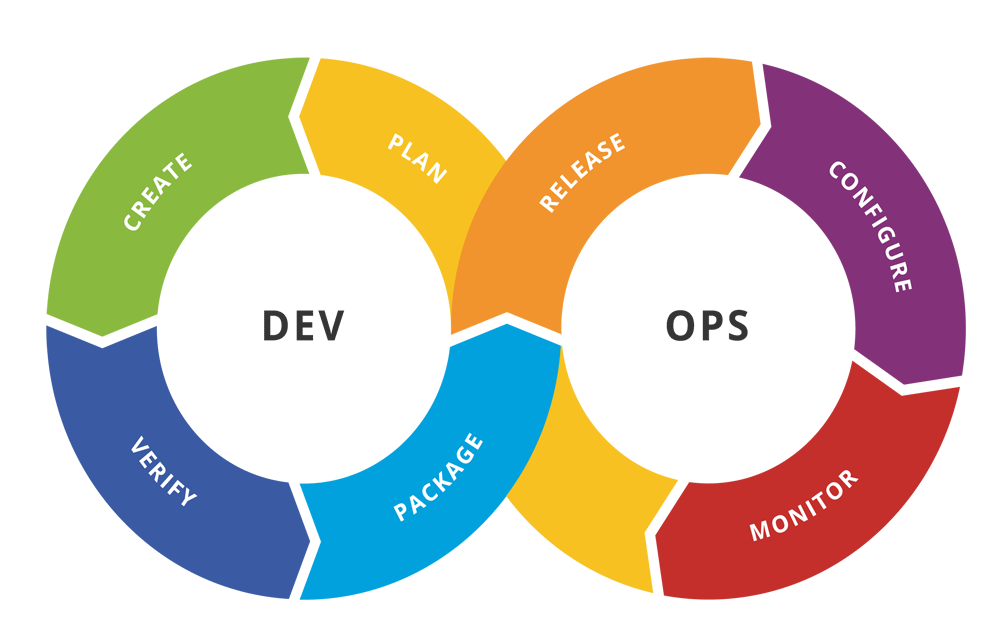
\includegraphics[width=\imagewidth]{DevOps.png}
        \caption{Source: \url{infolytx.com}}
        \end{figure}
        \vfill
     
            
        
            
        
            
        \Large
        Software development\\
        IT-University of Copenhagen\\
        Denmark\\
        June 1, 2022
            
    \end{center}
\end{titlepage}


\newpage
\thispagestyle{empty}
\tableofcontents
\thispagestyle{empty}
\newpage
\setcounter{page}{1}
\section{Introduction}
This report details our approach to designing, developing, and maintaining the ITU-minitwit system while learning DevOps practices in the course \textit{DevOps, Software Evolution, and Software Maintenance}.

The report's content is divided into three sections. The first section, \textit{System's Perspective}, describes the system's design and architecture, as well as its dependencies and licenses. The second section, \textit{Process' Perspective}, revolves around developer interactions, project organization, CI/CD, and security, among other relevant topics. The third section, \textit{Lessons Learned Perspective}, discusses the experiences and knowledge gained throughout the project. 

\bigskip
\noindent 
\href{https://github.com/aske-w/itu-minitwit}{\textbf{Project repository: https://github.com/aske-w/itu-minitwit}}

\section{System's Perspective}

% A description and illustration of the:

% 3+1 model: https://pure.au.dk/portal/files/15565758/christensen-corry-marius-2007.pdf

% Louise rapport: https://github.com/lauralunddahl/DevOps-GroupF/blob/master/report/report.md

\subsection{ Design and Architecture of your ITU-MiniTwit systems}
In this section we will show the design and architecture of the systems we implemented. To do this we use the 3+1 model by Christensen et al. \cite{christensen2004approach}.

%https://drive.google.com/file/d/1mVw5aNr07rwvz9QBqgGFAGrMUgVoj9QP/view?usp=sharing

\subsubsection{Module viewpoint}
The module viewpoint is visualized with a package diagram. This can be seen in figure \ref{fig:package-diagram}.

\begin{figure}[H]
   \centering
   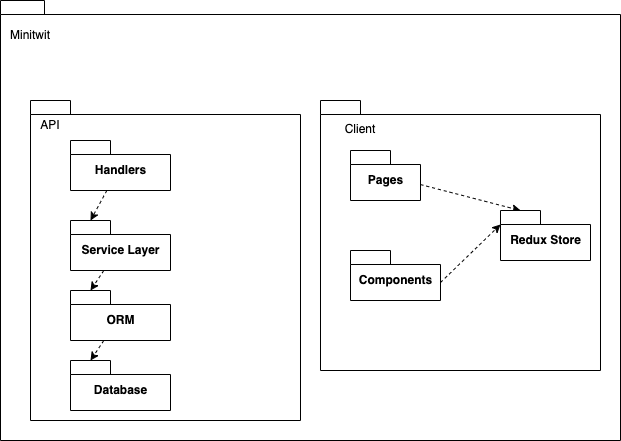
\includegraphics[width=\textwidth]{minitwit-system-architecture-1-packages.drawio.png}
   \caption{Shows the different packages for the API (server) and the Client (web application).}
   \label{fig:package-diagram}
\end{figure}

\subsubsection{Component \& Connector viewpoint}
Figure \ref{fig:c-and-c-diagram} shows the components of our system and how they can be accessed with HTTP from the browser.

\begin{figure}[H]
   \centering
   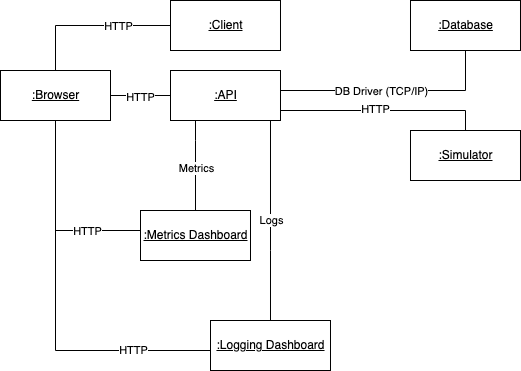
\includegraphics[width=\textwidth]{minitwit-system-architecture-1-components and connectors.drawio.png}
   \caption{Diagram over our components and how they connect with each other.}
   \label{fig:c-and-c-diagram}
\end{figure}
\newpage
\subsubsection{Allocation viewpoint}
The allocation viewpoint concerns itself with the deployment of the systems. This can be seen in figure \ref{fig:deployment-diagram}.

\begin{figure}[H]
   \centering
   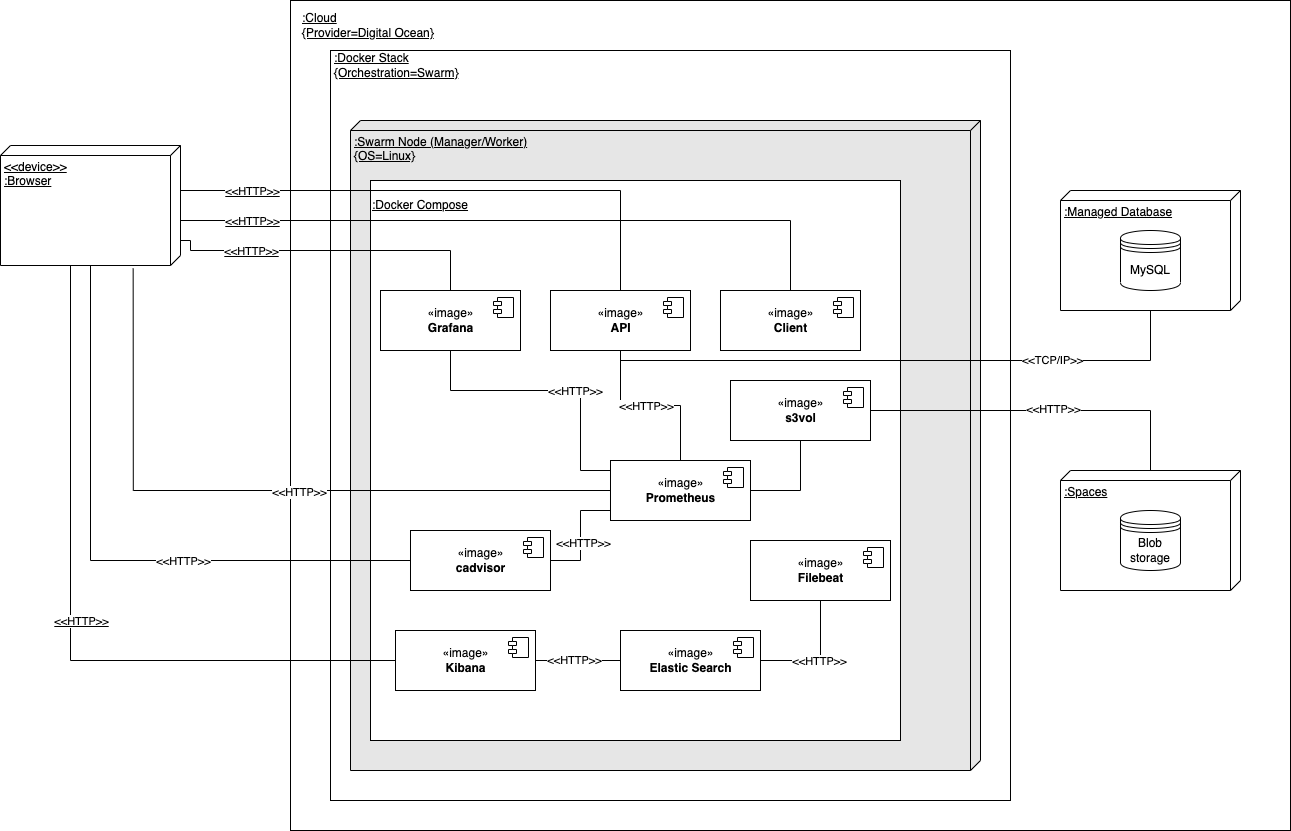
\includegraphics[width=\textwidth]{minitwit-system-architecture-1-deployment.drawio.png}
   \caption{Deployment diagram over the different items in our system.}
   \label{fig:deployment-diagram}
\end{figure}

\subsection{Dependencies}

We chose to replace the original Python implementation, with an implementation in Golang for the server application. Additionally, we split the application into server and client, and chose to implement the client in React. The dependencies associated with the client/server approach is listed below, alongside the dependencies associated with logging \& monitoring, infrastructure, and the development process.

\subsubsection{Backend application dependencies}
\begin{itemize}
    \item \href{https://github.com/kataras/iris}{\textbf{Iris}}: Go web framework.
    \item \href{https://gorm.io/}{\textbf{GORM}}: Object-relational mapper for Go, with MySQL and Prometheus drivers.
\end{itemize}

\subsubsection{Frontend application dependencies}
\begin{itemize}
    \item \href{https://reactjs.org/}{\textbf{React}}: JavaScript library for building user interfaces.
    \item \href{https://v5.reactrouter.com/}{\textbf{React-router-dom}}: Client based routing.
    \item \href{https://redux.js.org/}{\textbf{Redux}}: State management.
    \item \href{https://axios-http.com/docs/intro}{\textbf{Axios}}: HTTP client.
    \item \href{https://tailwindcss.com/}{\textbf{TailwindCSS}}: CSS framework.
\end{itemize}

\subsubsection{Logging \& Monitoring dependencies}
\begin{itemize}
    \item \href{https://github.com/google/cadvisor}{\textbf{cAdvisor}}: Container metrics.
    \item \href{https://prometheus.io/}{\textbf{Prometheus}}: Collecting monitoring data.
    \item \href{https://www.elastic.co/elasticsearch/}{\textbf{Elastic Search}}: Storing and search logs.
    \item \href{https://www.elastic.co/beats/filebeat}{\textbf{Filebeat}}: Export log collections to Elastic Search.
    \item \href{https://www.elastic.co/kibana/}{\textbf{Kibana}}: Visualization of logs in Elastic Search.
    \item \href{https://grafana.com/}{\textbf{Grafana}}: Dashboard to visualize Prometheus metrics.
\end{itemize}

\subsubsection{Infrastructure dependencies}
\begin{itemize}
    \item \href{https://www.digitalocean.com/products/droplets}{\textbf{DigitalOcean Droplet}}: Virtual machine instances.
    \item \href{https://www.digitalocean.com/products/managed-databases}{\textbf{DigitalOcean Managed Databases}}: MySQL database cluster with horizontal and vertical scaling of read-only nodes and vertical scaling for single write node (master).
    \item \href{https://hub.docker.com/}{ \textbf{Docker Hub}}: For storing and retrieving docker images.
\end{itemize}

\subsubsection{Development dependencies}
\begin{itemize}
    \item \href{https://git-scm.com/}{\textbf{Git}}: Distributed version control system
    \item \href{https://github.com/features/actions}{\textbf{Github Actions}}: Automatic actions for testing, analysis, deployment and releases.
\end{itemize}

\subsection{Important interactions of subsystems}
To show the interactions of the subsystems, we used the action of a client posting a message as an example. This shows how the different subsystems of Client, API, Logging, Database and Metrics interact in a typical scenario, which is visualized in a sequence diagram in figure \ref{fig:sequence-diagram}.

\begin{figure}[H]
   \centering
   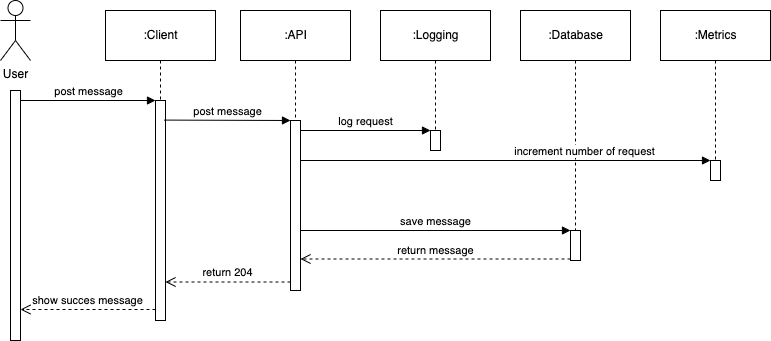
\includegraphics[width=\textwidth]{minitwit-system-architecture-1-sequence diagram.drawio.png}
   \caption{Sequence diagram over the action of \textit{posting a message}.}
   \label{fig:sequence-diagram}
\end{figure}


\subsection{Static analysis and quality assessment}

To ensure a certain level of quality within the repository, various tools for static analysis have been used. Every time a pull request is made to the \textit{development} branch, a GitHub Action is run. This action use the following tools \textit{gofmt}, \textit{gosec}, \textit{vet} and \textit{lichen}.
\textit{Gofmt} formats the code programmatically to ensure consistency. Vet checks the code for errors that the compiler might not find. \textit{Gosec} scans the binary for potential security vulnerabilities. Without the tools above running from the command-line, we also integrated with third-party tools \textit{SonarCloud}, \textit{Code Climate} and \textit{Better Code Hub}. The tools mostly show no problems related to the Go application. 
However, certain warnings are caused by the simulator and the original Python implementation, which are both included in the repository. The following are some of the areas that can be improved. Badges for overview can be seen in appendix \ref{appendix:static_analysis}.

\begin{itemize}
    \item Explicit error handling everywhere.
    \item Reduce cognitive complexity and length of some functions.
\end{itemize}

\noindent Our API has throughout the project been among the fastest, as seen in the figure \ref{fig:latest-chart}.

\begin{figure}[H]
   \centering
   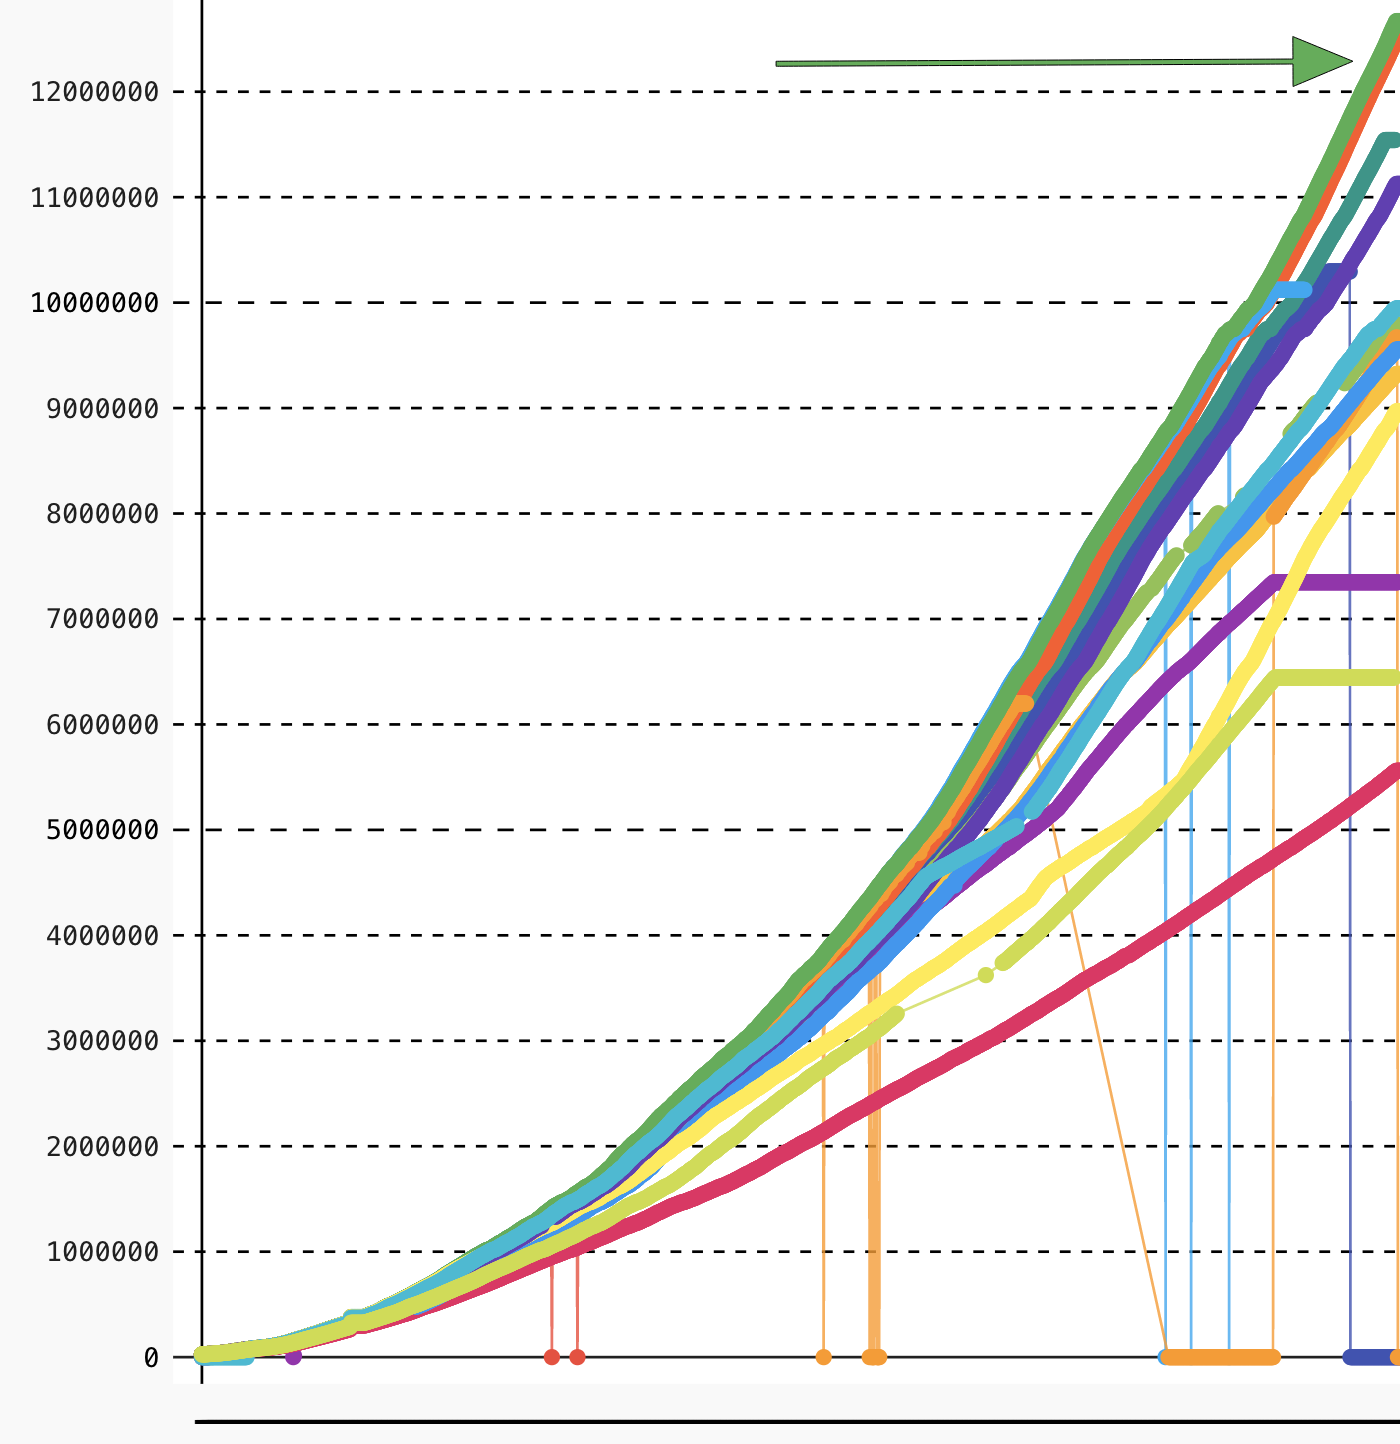
\includegraphics[width=\textwidth/2]{latest-chart.png}
   \caption{Latest number returned by the API. The green line, which the arrow points to, is ours.}
   \label{fig:latest-chart}
\end{figure}

A few times, we had issues with our database giving the error \textit{failed to read auto-increment value from storage engine}. This resulted in errors being thrown from our application as seen in figure \ref{fig:error-chart}. We fixed the error and since then, no errors have been returned from the API.

\begin{figure}[H]
   \centering
   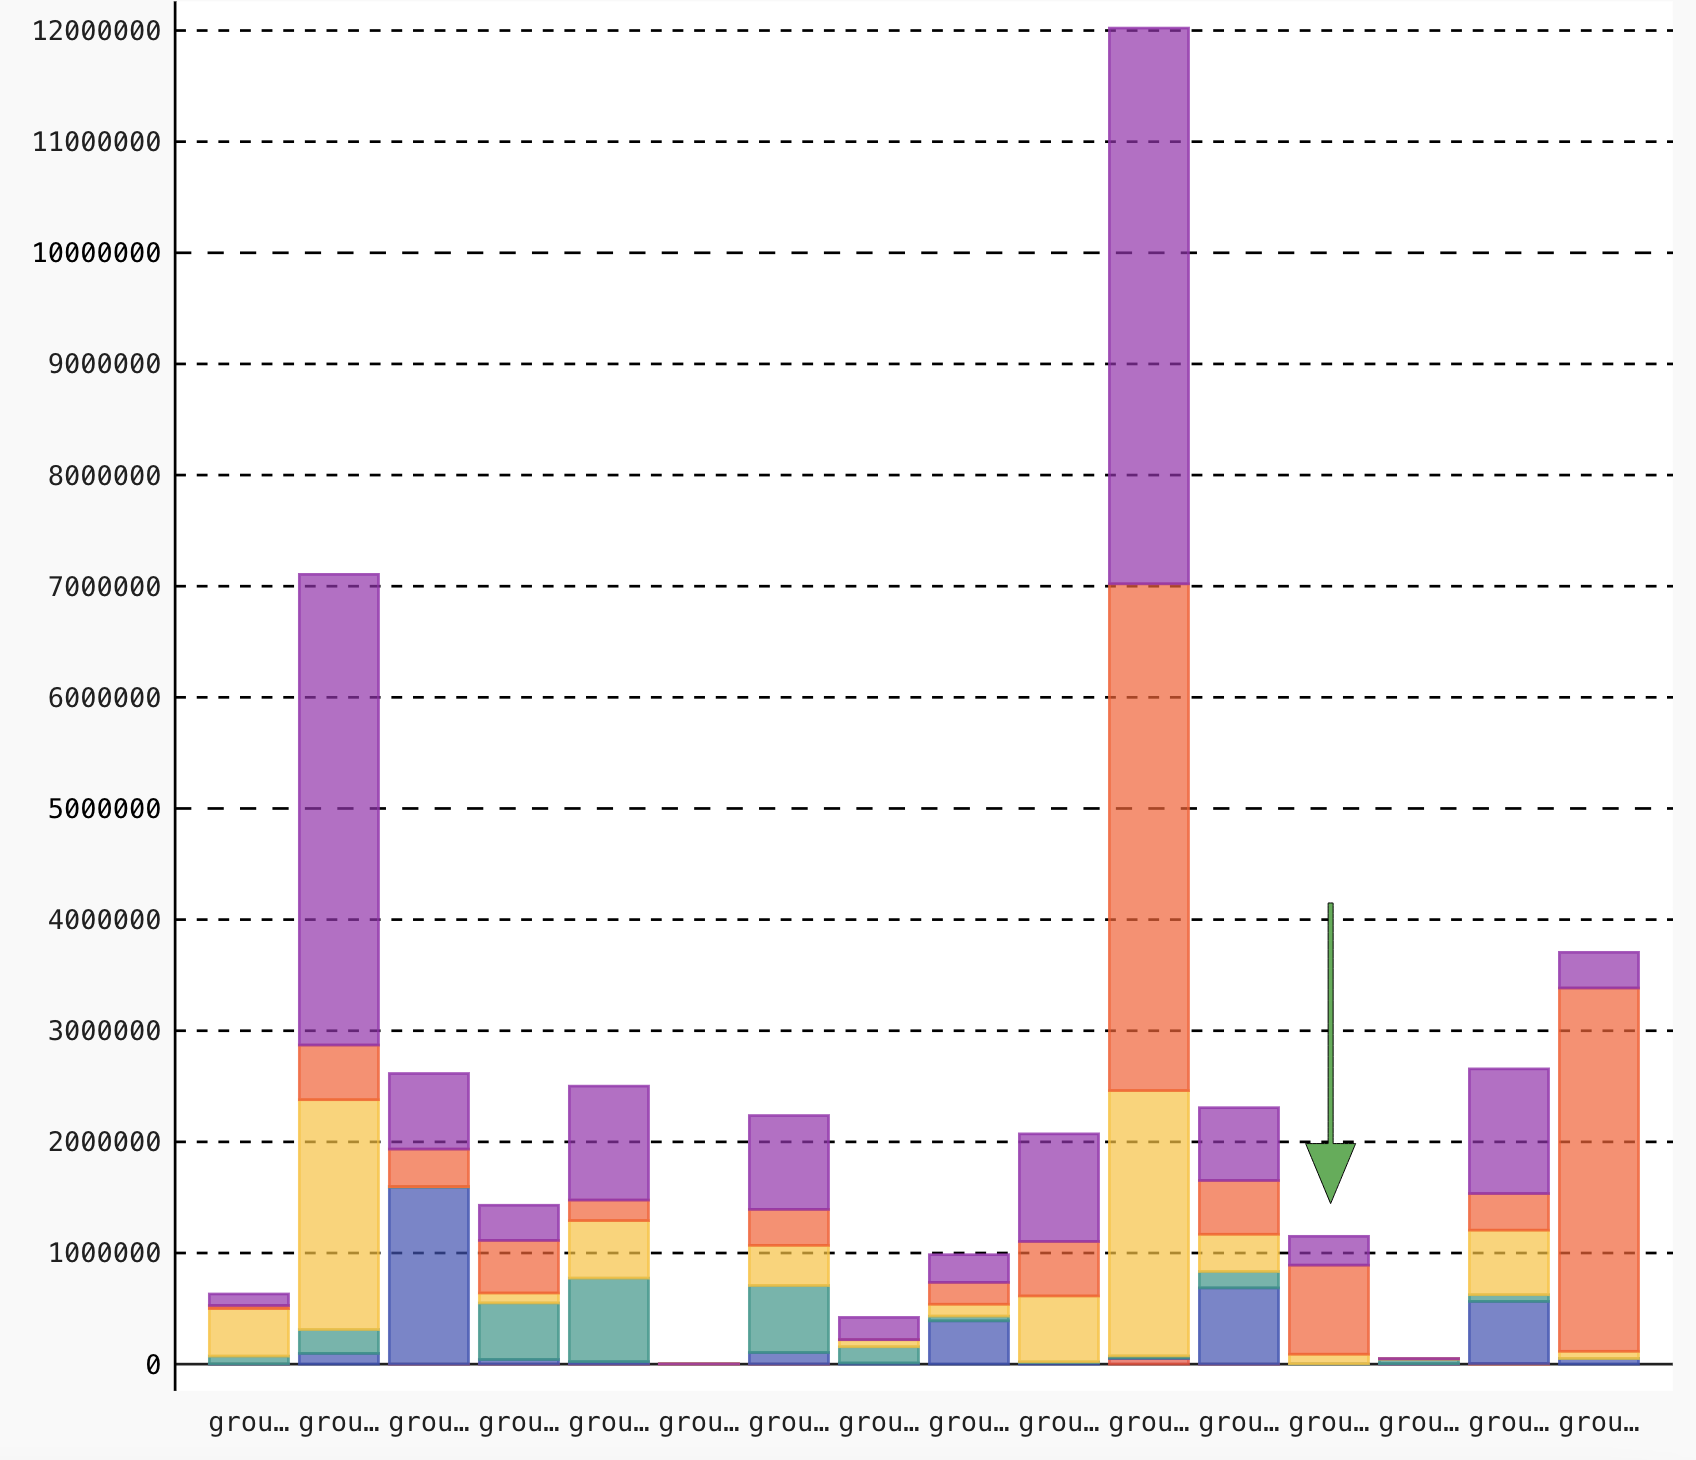
\includegraphics[width=\textwidth/2]{error-chart.png}
   \caption{Errors returned by the API. The green arrow shows ours.}
   \label{fig:error-chart}
\end{figure}



\subsection{License}
We chose the MIT license, which is a permissive license that is commonly used with open-source software. We use a Go package called \textit{Lichen} to check if we are compliant with the licenses of our dependencies. This has been implemented as a Github Action CI/CD check. The MIT license is compliant with all of our dependencies, which can be seen in appendix \ref{appendix:lichen-output}.



\section{Process' perspective}


\subsection{Developer interactions and teamwork}


%notes
\noindent Throughout the project, we have held meetings alongside development in person every Tuesday, following the weekly lectures in the course. In between these meetings, we have resorted to using Facebook Messenger and Discord for asynchronous communication.
Usually, the group has been divided into sub-groups of developers, dependent on the complexity of the work.


\subsection{CI/CD}
We use GitHub Actions as our continuous integration and continuous delivery platform. We have three separate workflows/pipelines configured, that run independently of each other. Pull requests to our development branch will trigger the test workflow. This workflow will run all tests against the development branch. We also run a static analysis workflow concurrently with the test workflow. Static analysis includes multiple steps. Initially, the code is formatted and then vetted for suspicious elements. Afterwards, a security scanner will check the entire code base for security flaws. Finally, we scan all of our dependencies' licenses to ensure we are using these dependencies under their license agreements. If any steps fail, the entire workflow will render itself a failure. We will only be able to merge the pull request into the development branch if both workflows succeed.

When pull requests have been merged into the development branch, we can deploy the changes by creating another pull request from the development branch to the main branch. This will trigger the deployment workflow. The deployment workflow includes a few steps:
\begin{enumerate}
    \item Checkout the code
    \item Authenticate with Docker Hub
    \item Build and push a new tagged docker image for the server to Docker Hub
    \item Build and push a new tagged docker image for the client to Docker Hub
    \item Copy ./swarm/docker-compose.yml, ./swarm/filebeat.yml, ./swarm/grafana/ and ./swarm/prometheus/ to the server using SSH
    %\item Copy ./swarm/filebeat.yml to the server using SSH
    \item SSH into worker server and ensure correct permissions
    \item SSH into server and pull the newly pushed images from Docker Hub and deploy the swarm
    \item Tag the commit and create a GitHub release with a change log
\end{enumerate}

\subsection{Organization of repository and branching}
We use a mono-repository structure to store all of our code and assets. The client and server code is split into separate folders within the same repository. The repository also contains configuration folders for Filebeat, Grafana and Prometheus.

\subsubsection{Branching Strategy}
We have chosen to keep our branching strategy simple with the Git-flow branching strategy combined with a locked main branch. This means that nobody can push directly to it. Every change to the main branch must be made through pull requests from the development branch. All pull requests to the main branch are required to be reviewed by at least one collaborator before it can be merged. It must also pass all automated actions.

The development branch should always be either ahead of main or up-to-date with main. When developing new features, collaborators branch out from development and later create a pull request to development. Basically, we have the following branches: main, development, hotfix/*, and feature/*.

The \textit{main} branch is used as production, and a \textit{development} branch is used for development. A new feature will be worked on in a separate \textit{feature} branch that is branched out from \textit{development}. When a feature is complete, the associated branch is merged into \textit{development}. The \textit{main} branch will pull from development to release stable changes to \textit{production}. We used the naming convention of prepending \textit{feature/*} and \textit{hotfix/*} to distinguish between feature and hotfix branches.

\begin{figure}[H]
   \centering
   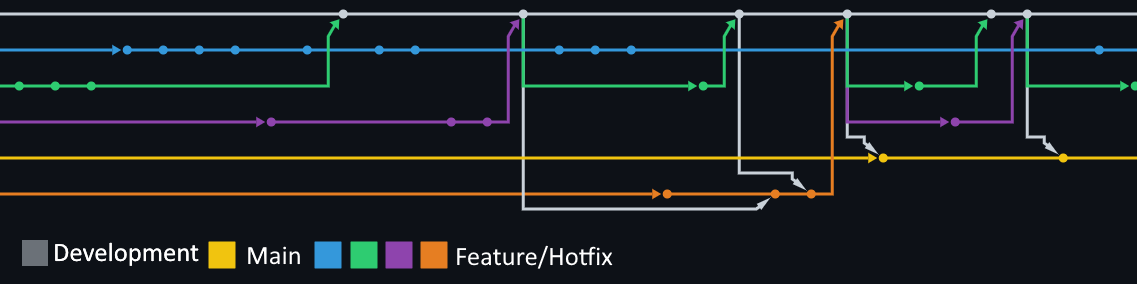
\includegraphics[width=\textwidth]{branching.png}
   \caption{Visualized network graph of branches from Github. The graph shows the \textit{main} branch (yellow), \textit{development} (grey) and various \textit{feature} and \textit{hotfix} branches (blue, green, purple, orange). The graph shows how features and hotfixes are merged into development before being merged into production. The graph also shows that some features or hotfixes have been merged with development to minimize merge conflicts.}
   \label{fig:my_label}
\end{figure}

\subsection{Development process}
%  \textit{ Applied development process and tools supporting it}
%     \begin{itemize}
%         \item \textit{For example, how did you use issues, Kanban boards, etc. to organize open tasks.}
%     \end{itemize}

\noindent We have used the Projects feature, essentially a Kanban board, on GitHub to handle the organization of the work that is to be done \ref{fig:githubprojects}. The reasoning behind this, was to centralize our workflow as much as possible. Whenever a task had been defined during a meeting, we would add the task and assign the person(s) responsible for it.
\begin{figure}[H]
   \centering
   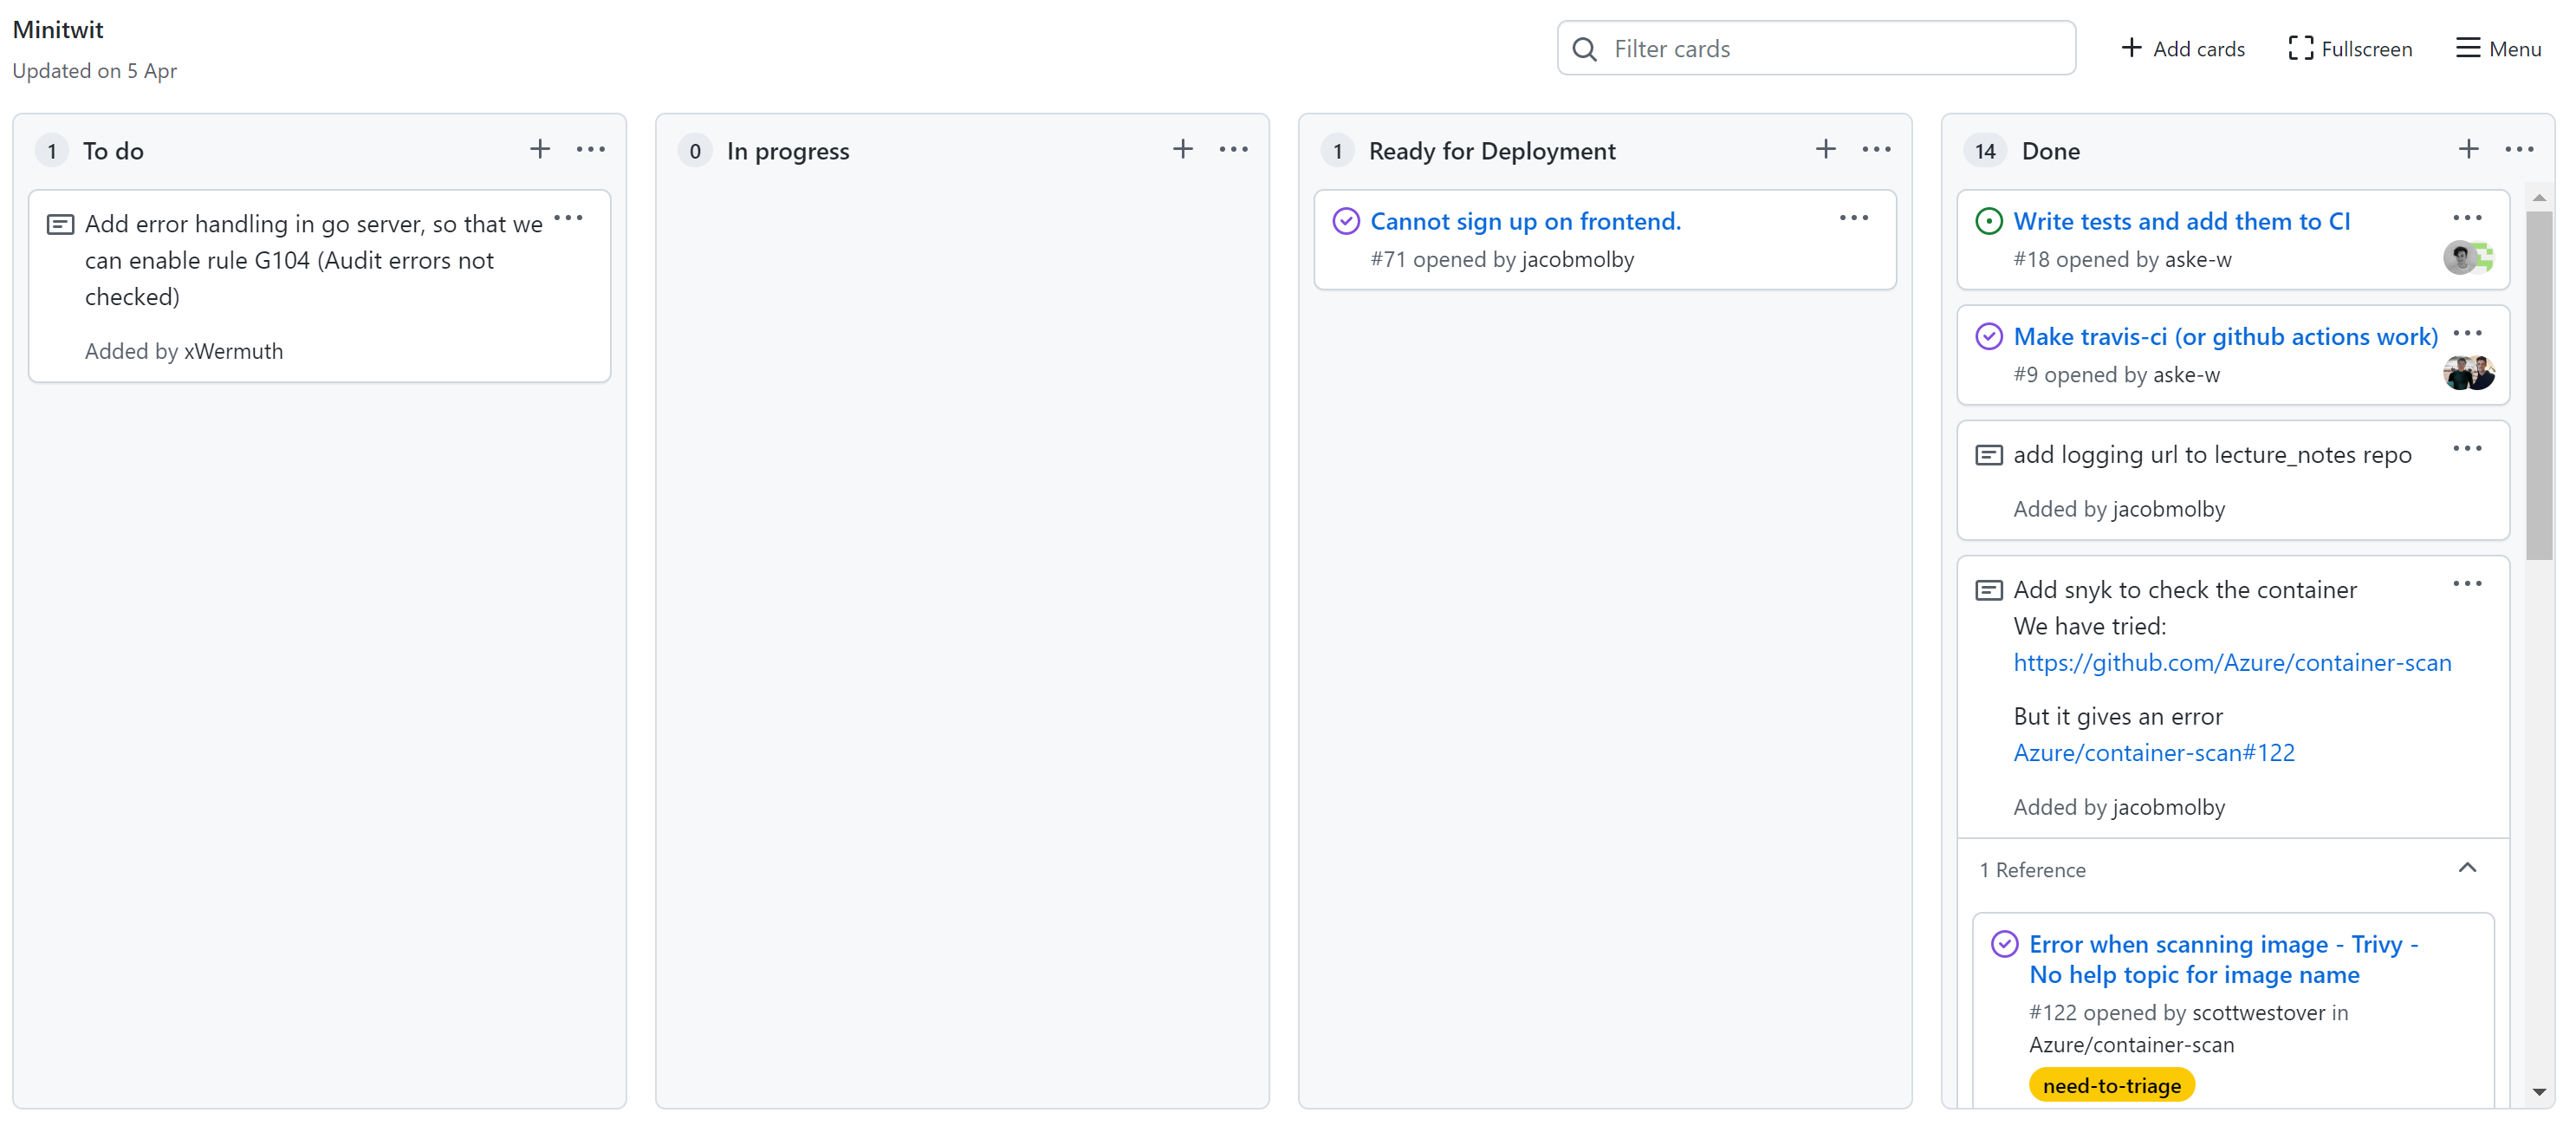
\includegraphics[width=\textwidth]{GitHubProjects.png}
   \caption{GitHub Projects for organization of tasks.}
   \label{fig:githubprojects}
\end{figure}

\subsection{Monitoring and logging}

\subsubsection{Logging}
For logging, we use the EFK-stack that consists of the following three elements Elastic, Filebeat and Kibana. The EFK-stack is a way of aggregating large volumes of logs to quickly sort through and analyze them \cite{elk-stack}. This is especially helpful if a significant part of the infrastructure is hosted in the cloud.
\\
Filebeat collects, transforms, and ships logs to the ElasticSearch back end \cite{filebeat}. Furthermore, Filebeat is used to configure an index for ElasticSearch. In our case, we created an index on the Docker container running our server to filter by its logs and not get overwhelmed by the other containers' logs. In Kibana the logs are visualized, where we can filter by multiple fields such as timestamp, log type (error, warning, etc.), and many others \cite{kibana}.

Figure \ref{fig:log-stack} shows our logging infrastructure.

\begin{figure}[H]
   \centering
   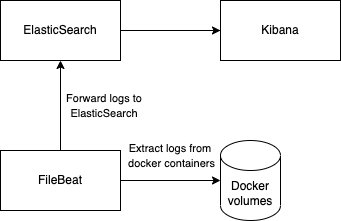
\includegraphics[width=\imagewidth/2]{Logging.drawio.png}
   \caption{Simple overview of our ELK-stack}
   \label{fig:log-stack}
\end{figure}

If we wanted to have our logs more structured, we might have considered including Logstash in our stack. That would have made the logs easier to analyze. Logstash like Filebeat can also send data to ElastichSearch, but it also acts as an aggregator, where it pulls data from various sources and transform the data into meaningful logs before pushing it to ElasticSearch \cite{filebeat-vs-logstash}. However, Logstash processing has the disadvantage of being slow and since our infrastructure is small, enhancing the logs is not needed. 

\subsubsection{Monitoring}
Grafana and Prometheus are used for monitoring our application. Prometheus is used to store the collected metrics, and Grafana is used as the interface for visualizing the data. We are monitoring metrics within four different categories: Web Server, Container Statistics, Database and Business Intelligence. The metrics monitored are listed below. Screenshots of the dashboard can be seen in appendix \ref{monitoring_dashboard}.

\textbf{Web Server:}
\begin{itemize}
    \item Simulator endpoints response time
    \item Regular endpoints response time
    \item Number of accesses to endpoints
\end{itemize}

\textbf{Container Statistics:}
\begin{itemize}
    \item CPU usage 
    \item Memory usage
\end{itemize}

\textbf{Database:}
\begin{itemize}
    \item Uptime
    \item Active connections
    \item Idle connections
    \item Number of threads running
    \item Number of slow queries
\end{itemize}

\textbf{Business Intelligence:}
\begin{itemize}
    \item Average followers per user
    \item Total number of users
\end{itemize}


% \textit{How do you monitor your systems and what precisely do you monitor?}
% \textit{What do you log in your systems and how do you aggregate logs?}

\subsection{Security}
In this section we will describe the results of our security assessment.
\subsubsection*{Risk Identification}
We identified the following assets that could be vulnerable.
\begin{itemize}
    \item API/server (Go application)
    \item Webclient (React.js application, served with NGINX)
    \item Graphana
    \item Prometheus
    \item cAdvisor
    \item Elastic Search
    \item Kibana
    \item Filebeat
    \item MySQL database
\end{itemize}

\noindent For these assets certain threat sources were also identified:

\begin{enumerate}
    \item SQL injection on web client.
    \item XSS on web client.
    \item Malicious actor accessing secrets.
    \item DDoS on VPS.
    \item Hacker guessing the passwords of users.
\end{enumerate}

\noindent Based on the threat sources different risk scenarios where devised.

\begin{enumerate}
    \item Attacker performs SQL injection to download or destroy data from the database.
    \item Attacker inputs JavaScript in an input field and accesses data of another user.
    \item Attacker is able to socially engineer a group member to expose a secret.
    \item Attacker uses DDoS to crash or halt our server or database.
    \item Since we have no requirements for passwords, it is possible for the users to create single letter or number passwords. This would make it very easy for the attacker to exploit using a dictionary or brute force attack.
\end{enumerate}

\subsubsection*{Risk Analysis}
Based on the identification of risks above, we conducted a risk analysis. For this purpose, a risk matrix has been constructed as seen in table \ref{tab:risk-matrix}. The matrix consists of likelihoods on the x-axis and impacts on the y-axis. Each of the scenarios from above has been inserted based on their likelihood and impact.

\begin{table}[H]
\centering
\begin{tabular}{clcllll}
\multicolumn{1}{l}{}                                    &                                    & \multicolumn{5}{c}{\textbf{Likelihoods}}                                                                                                                                                                                                                                                       \\ \cline{2-7} 
\multicolumn{1}{l|}{}                                   & \multicolumn{1}{l|}{}              & \multicolumn{1}{l|}{Rare}                               & \multicolumn{1}{l|}{Unlikely}                           & \multicolumn{1}{l|}{Possible}                           & \multicolumn{1}{l|}{Likely}                            & \multicolumn{1}{l|}{Certain}                            \\ \cline{2-7} 
\multicolumn{1}{c|}{}                                   & \multicolumn{1}{l|}{Catastrophic}  & \multicolumn{1}{c|}{\cellcolor[HTML]{F8FF00}\textbf{}}  & \multicolumn{1}{c|}{\cellcolor[HTML]{FFC702}\textbf{1}} & \multicolumn{1}{c|}{\cellcolor[HTML]{FE0000}\textbf{}}  & \multicolumn{1}{c|}{\cellcolor[HTML]{FE0000}\textbf{}} & \multicolumn{1}{c|}{\cellcolor[HTML]{FE0000}\textbf{}}  \\ \cline{2-7} 
\multicolumn{1}{c|}{}                                   & \multicolumn{1}{l|}{Critical}      & \multicolumn{1}{c|}{\cellcolor[HTML]{F8FF00}\textbf{3}} & \multicolumn{1}{c|}{\cellcolor[HTML]{FFC702}\textbf{}}  & \multicolumn{1}{c|}{\cellcolor[HTML]{FFC702}\textbf{2}} & \multicolumn{1}{c|}{\cellcolor[HTML]{FE0000}\textbf{}} & \multicolumn{1}{c|}{\cellcolor[HTML]{FE0000}\textbf{5}} \\ \cline{2-7} 
\multicolumn{1}{c|}{}                                   & \multicolumn{1}{l|}{Marginal}      & \multicolumn{1}{c|}{\cellcolor[HTML]{32CB00}\textbf{}}  & \multicolumn{1}{c|}{\cellcolor[HTML]{F8FF00}\textbf{}}  & \multicolumn{1}{c|}{\cellcolor[HTML]{FFC702}\textbf{4}} & \multicolumn{1}{c|}{\cellcolor[HTML]{FFC702}\textbf{}} & \multicolumn{1}{c|}{\cellcolor[HTML]{FE0000}\textbf{}}  \\ \cline{2-7} 
\multicolumn{1}{c|}{}                                   & \multicolumn{1}{l|}{Negligible}    & \multicolumn{1}{l|}{\cellcolor[HTML]{32CB00}}           & \multicolumn{1}{l|}{\cellcolor[HTML]{F8FF00}}           & \multicolumn{1}{l|}{\cellcolor[HTML]{F8FF00}}           & \multicolumn{1}{l|}{\cellcolor[HTML]{FFC702}}          & \multicolumn{1}{l|}{\cellcolor[HTML]{FFC702}}           \\ \cline{2-7} 
\multicolumn{1}{c|}{\multirow{-5}{*}{\rotatebox{90}{\textbf{Impacts}}}} & \multicolumn{1}{l|}{Insignificant} & \multicolumn{1}{l|}{\cellcolor[HTML]{32CB00}}           & \multicolumn{1}{l|}{\cellcolor[HTML]{32CB00}}           & \multicolumn{1}{l|}{\cellcolor[HTML]{32CB00}}           & \multicolumn{1}{l|}{\cellcolor[HTML]{F8FF00}}          & \multicolumn{1}{l|}{\cellcolor[HTML]{F8FF00}}           \\ \cline{2-7} 
\end{tabular}
\caption{Risk matrix for the scenarios. The numbers indicate a scenario from above.}
\label{tab:risk-matrix}
\end{table}

\noindent To mitigate the risk the following is planned to safeguard against possible attacks.
\begin{itemize}

  \item \textbf{Scenario 1:} Fix the injections and restore backups.
  \item \textbf{Scenario 2:} Issue an apology to the user and fix the injections.
  \item \textbf{Scenario 3:} Give the exposed group member a security course and change all secrets.
  \item \textbf{Scenario 4:} Restart the server. Setup DDoS protection like a firewall or CloudFlare.
  \item \textbf{Scenario 5:} Reset the users' password. To mitigate future attacks, we should implement minimum requirements for the passwords on user creation.
  
\end{itemize}
 
 
 
We also did a penetration test. With tools available in the Kali Linux distribution we tried a variety of automated penetration tools like \texttt{wmap}, \texttt{nmap} and \texttt{metasploit}. None of them were successful in having an impact on our system.

\subsection{Scaling and load balancing strategy}
% \textit{Applied strategy for scaling and load balancing.}

During the course we have applied different strategies for scaling our Minitwit application. We were able to use the smallest droplet available on DigitalOcean until the implementation of logging with the EFK-stack. We had to scale vertically since we needed more RAM. 

After the lecture on \textit{deployment strategies, scalability and load balancing} we implemented the ability to scale horizontally for high availability for the Minitwit application. We discovered Docker Stack which allows you to deploy a compose file into a swarm. We used Docker Swarm as an orchestrator to distribute our services between two nodes. Then the manager node schedules the services as replica tasks on nodes in the swarm \cite{docker-swarm-docs}.

We have not defined any services to be replicated for load balancing. Nevertheless, some services are replicated on all nodes out of necessity, such as \textit{cAdvisor}, which collects container data for containers running on a node. \textit{Filebeat} is also replicated on all nodes to pull logs from the containers on each node.

Docker Swarm's routing mesh obfuscates container placement from the point of view of requests and automatically routes requests to nodes with the requested containers. If we had automatically scaled the services, the routing mesh would automatically load balance requests between nodes and containers.

%Docker Swarm Routing mesh....


\section{Lessons Learned Perspective}

% Describe the biggest issues, how you solved them, and which are major lessons learned with regards to:

% \begin{itemize}
%     \item evolution and refactoring
%     \item operation, and
%     \item maintenance
% \end{itemize}

% of your ITU-MiniTwit systems. Link back to respective commit messages, issues, tickets, etc. to illustrate these. Also reflect and describe what was the "DevOps" style of your work. For example, what did you do differently to previous development projects and how did it work?

\subsection{Testing \& Splitting Web Client and API}

\noindent We chose to split the Web Client from the API to conduct tests on the API. Before this, our tests revolved around asserting the text embedded in the HTML, which the API would serve. This also allowed us to change the authentication to JSON Web Tokens, which simplified testing compared to the previous authentication, that used cookies stored in sessions (see pull request \href{https://github.com/aske-w/itu-minitwit/pull/89}{{\#89}}).

\subsection{ElasticSearch}
% elastic search is RAM intensive which is expensive. Datadog is less intensive
In our current setup, we have two servers with 4GB of memory each. Ideally, we would have at least three servers running to increase resilience. However, the ElasticSearch image in Docker uses at least 2GB of memory and our free credits in DigitalOcean can only afford two servers with 4GB of memory. 

If we wanted to have three servers running, we could have used a managed service like Datadog for log management. Especially, since our infrastructure is small, it could be unnecessary with the ELK-stack, since we do not use many of its features. 

\subsection{GitGuardian}
GitGuardian was a helpful tool to alert if secrets were committed by accident. The alerts were sometimes false positives, however, it did successfully detect the inclusion of secrets in the commit \href{https://github.com/aske-w/itu-minitwit/commit/d7e4d9b96f1ee629949f01fc11580a61edf16e92#diff-1814a5376f0ff1c06a3246d8f862309b7539f129dfd197ae73f95c8f87750678R8}{d7e4d9b}.

GitGuardian sent an email to the repository owner since the repository was not set up as a team, with a notification of a possible secret exposure. The email can be seen in appendix \ref{fig:gitguardian_email}
The alert helped us minimize the time in which the secrets were exposed. Otherwise, we might never have noticed the exposure.

To mitigate malicious use, the secrets were changed as soon as we noticed the alert. Further, we added the directory in which the files with the secrets were in to our \texttt{.gitignore}, as they were not necessary to commit anyway.

\subsection{Persistence of Prometheus Data}

It did not occur to us before the end of April that saving the monitoring data from Prometheus was a good idea, especially to show this data at the exam. Furthermore, in a real-life production setting, you might want to have historical monitoring data, to some extent, to accompany your logging data.

To persist this data was a relatively simple exercise. We created a volume to map the directory in which Prometheus saves its data inside its container to a directory on the host machine. Then, we used a container called \texttt{s3vol} to store the directory on the host machine in a blob storage at DigitalOcean. This was done by creating a volume mapping the host directory to the directory in s3vol which it sends to the blob storage. The persistence of Prometheus data can be seen in commit \href{https://github.com/aske-w/itu-minitwit/commit/11844f8c0af04ecdc5992681cdda0c5ea357a6d8}{11844f8}.

%\subsection{Travis CI}
%Initially, we used Travis CI for Continues Deployment because it was recommended in the course. However, we found it difficult to setup and it was not free. Therefore, we decided to switch to GitHub Actions.

\subsection{Terraform}
At the beginning of the project, Vagrant was used to provision the server. However, we could not provision Docker Swarm with Vagrant, as some unsolvable errors kept occurring. Therefore, we switched to provisioning via bash scripts. However, bash scripts are imperative and can be difficult to understand. Therefore, late in the project, we changed to use Terraform, which is written in a declarative language. It also provides features such as first-party integrations with cloud providers, drift detection and validation of the infrastructure. This can be seen in commit \href{https://github.com/aske-w/itu-minitwit/commit/3b0684ae4d10921b369ba92bf960bf13b54d7413}{3b0684a}.

\subsection{Logging}
In the current state of the application, logs are stored on the servers. However, if the servers restart the old logs will be overwritten, resulting in a loss of critical information. In addition, having the logs in one place presents a security issue. If an attacker gains access, the person can delete the logs and cover up his tracks. With externalized logs, it might help warn an attack is occurring and gives a better chance of preventing it. Therefore, it would preferable to send the logs to a blob storage like \texttt{s3vol} within a given interval. 
\\
Furthermore, to make sure additional critical logs are not deleted, we should also configure the default log rotation of ElasticSearch, where it creates a new log file each day and persists it for a week before deleting it \cite{elastic-log-rotation}. 

\subsection{DevOps Reflections}
This project has differentiated itself from other code projects, because of the focus on infrastructure and automation. Previous projects have mostly revolved around the development of new features. By automating the infrastructure and implementing continuous integration and continuous deployment, we were able to reduce the amount of time spent on integration and deployment. This allowed us to work more efficiently by deploying smaller increments more frequently, resulting in less merge conflict.

The DevOps Handbook characterize DevOps by three principles; flow, feedback and continual learning and experimentation \cite[Ch. 1-4]{Kim2016-st}. 

Our workflow followed all the characteristics of the flow principle. We could improve on making work more visible. We have a GitHub projects Kanban board, but it was not used much, since we immediately started doing the weekly assignments. It was more used for tracking long running tasks and bugs. We made small batches of work, which we deployed continuously. We had minimal handoffs since only our team worked on the Minitwit application. We reduced many constraints through automation of code deployment and testing. Using Docker allowed us to replicate the production environment locally, but could have been better since we had to use separate docker-compose files. 

For the feedback characteristic, we have not adhered to swarming to solve problems and build new knowledge. If one person struggled they have been able to get help from others, but we have not had a problem where all group members sat around one computer to solve it. To see problems as they occur, we have automated build and testing through GitHub Actions. Changes would automatically be rejected if these failed. We have used Grafana to monitor the state of our application. What we looked for, was if containers were online or using excessive amounts of resources, and how fast our simulator endpoints responded. We have always been the ones to make decisions and review others work, and therefore we have pushed quality close to the source, i.e. the evolution and maintenance of the Minitwit application. We have optimized our work for downstream work centers, i.e. ourselves, through a well-considered software architecture and contributing helpful information to our README.
\\
Our workflow does not exhibit the trait of continual learning and experimentation to the same extent as the other two characteristics of DevOps. We have not institutionalized the improvement of daily work by time boxing error fixes. Rather, we have fixed problems as they have occurred and written helpful information in the README. We also lack in terms of resilience patterns. We rely a lot on GitHub, but we are aware of the consequences of this. 

In terms of a learning culture, we have respected that some things have taken longer than others. Many of the concepts during the course have been new to us. Therefore, we have spend time understanding these concepts and adapting them for the Minitwit application. Even though it has been a source of frustration, we have all done tasks which turned out to be more difficult than anticipated.

\section{Conclusion}
Working on this project has emphasized the benefits of infrastructure and automation within software development. Automation saves time and resources and establishes structure, which is important when multiple developers are working on a project simultaneously. The structure also contributes to the stability of the system whenever new features or changes are deployed. The use of continuous integration and continuous deployments encourages faster and more frequent delivery, which helps ensure that written code actually gets deployed to production. Altogether, the practices of DevOps streamlines the development process while ensuring high quality software.

%* Automation (saves time and resources)
%* Needs a structure when working that many people together (also contributes to stability when a new a feature needs to be deployed)
%* The importance CI / CD (Maintaining stability) 
%* Faster and more frequent delivery = faster deployment
%* 

%streamline development by automation, 
%Learned the import lesson of automation. For example Terraform streamlines provisioning



\newpage
\printbibliography[ heading=bibintoc, title={References}]

\newpage
\appendix
\appendixpage
\addappheadtotoc
\addtocontents{toc}{\protect\setcounter{tocdepth}{1}}% This turns off subsections

\section{Figures}
\subsection{GitGuardian notification}
\begin{figure}[H]
   \centering
   
\includegraphics[height=\imagewidth]{gitguardian email.png}
   \caption{Email from GitGuardian notifying of secrets accidentally being commited}
   \label{fig:gitguardian_email}
\end{figure}

\subsection{Grafana monitoring dashboard screenshots}
\label{monitoring_dashboard}
For some monitoring measures the dashboard does not aggregate data correctly from different servers. Therefore, it may seem like there are 3 nodes instead of 2, and some data is duplicated.

\begin{figure}[H]
   \centering
   \rotatebox{90}{
        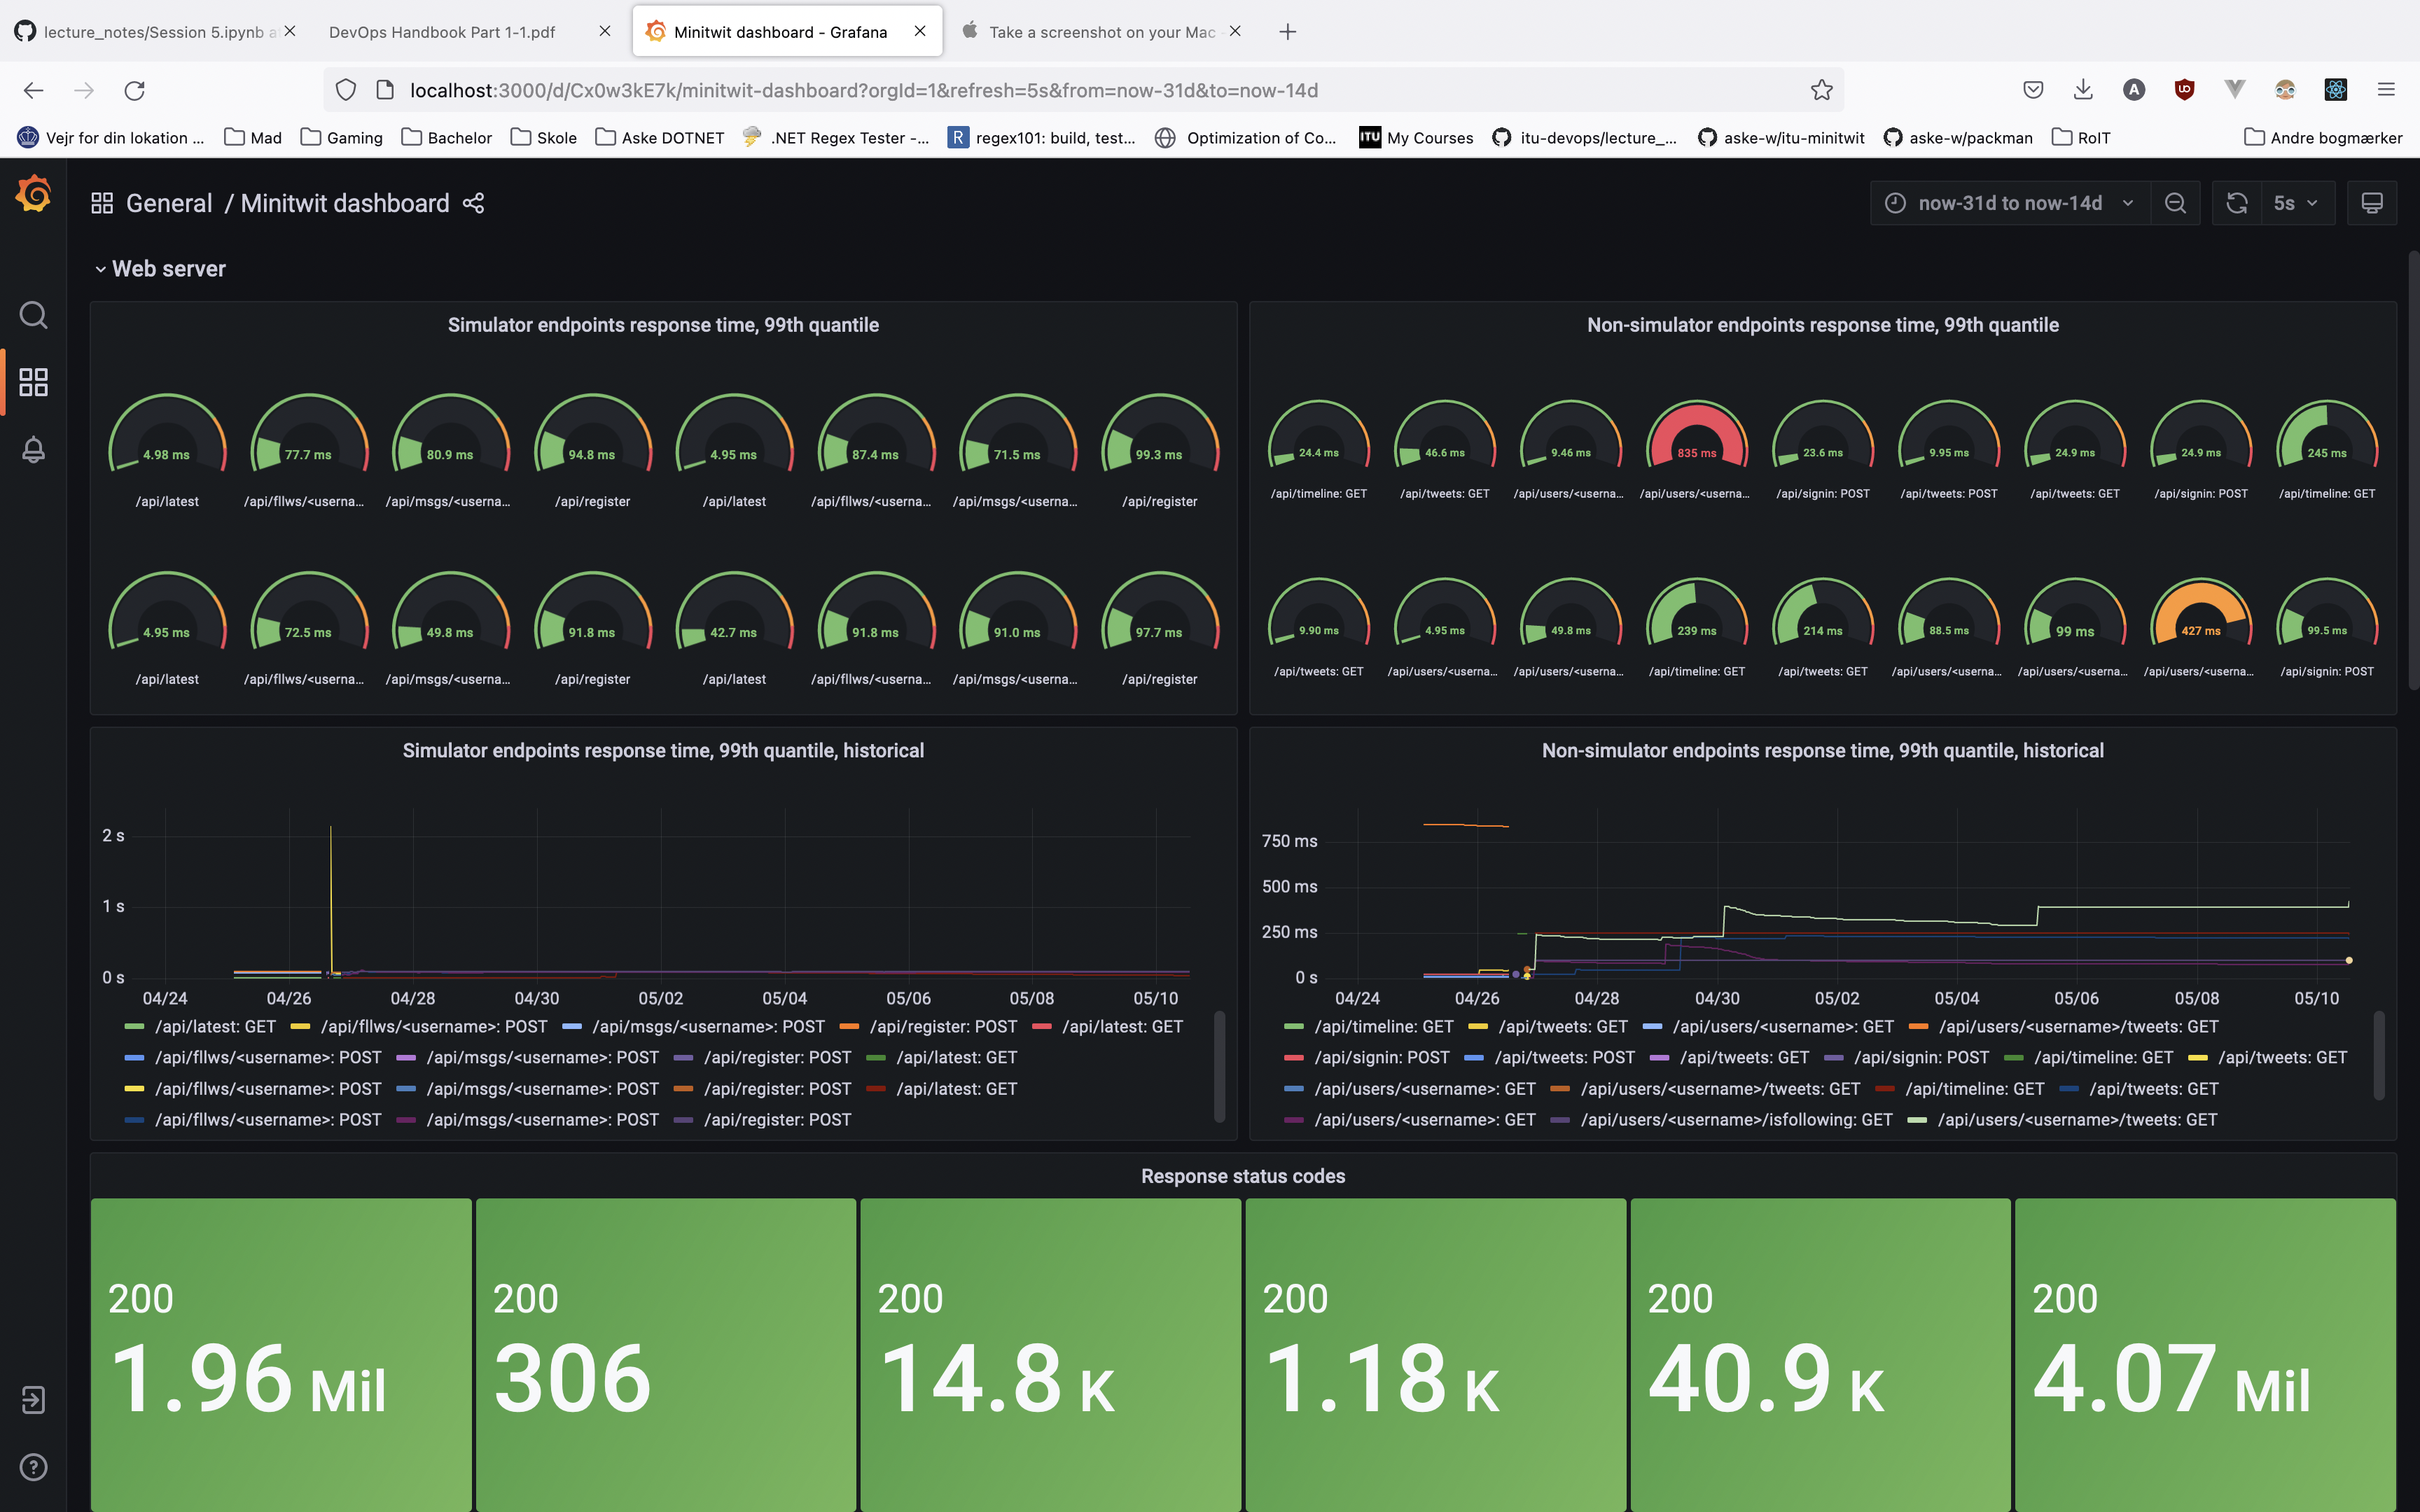
\includegraphics[height=0.6\textheight]{dashboard_1.png}
   }
   \caption{Screenshot of the Grafana dashboard showing endpoints response time and status codes}
   %\label{fig:gitguardian_email}
\end{figure}

\begin{figure}[H]
   \centering
   \rotatebox{90}{
        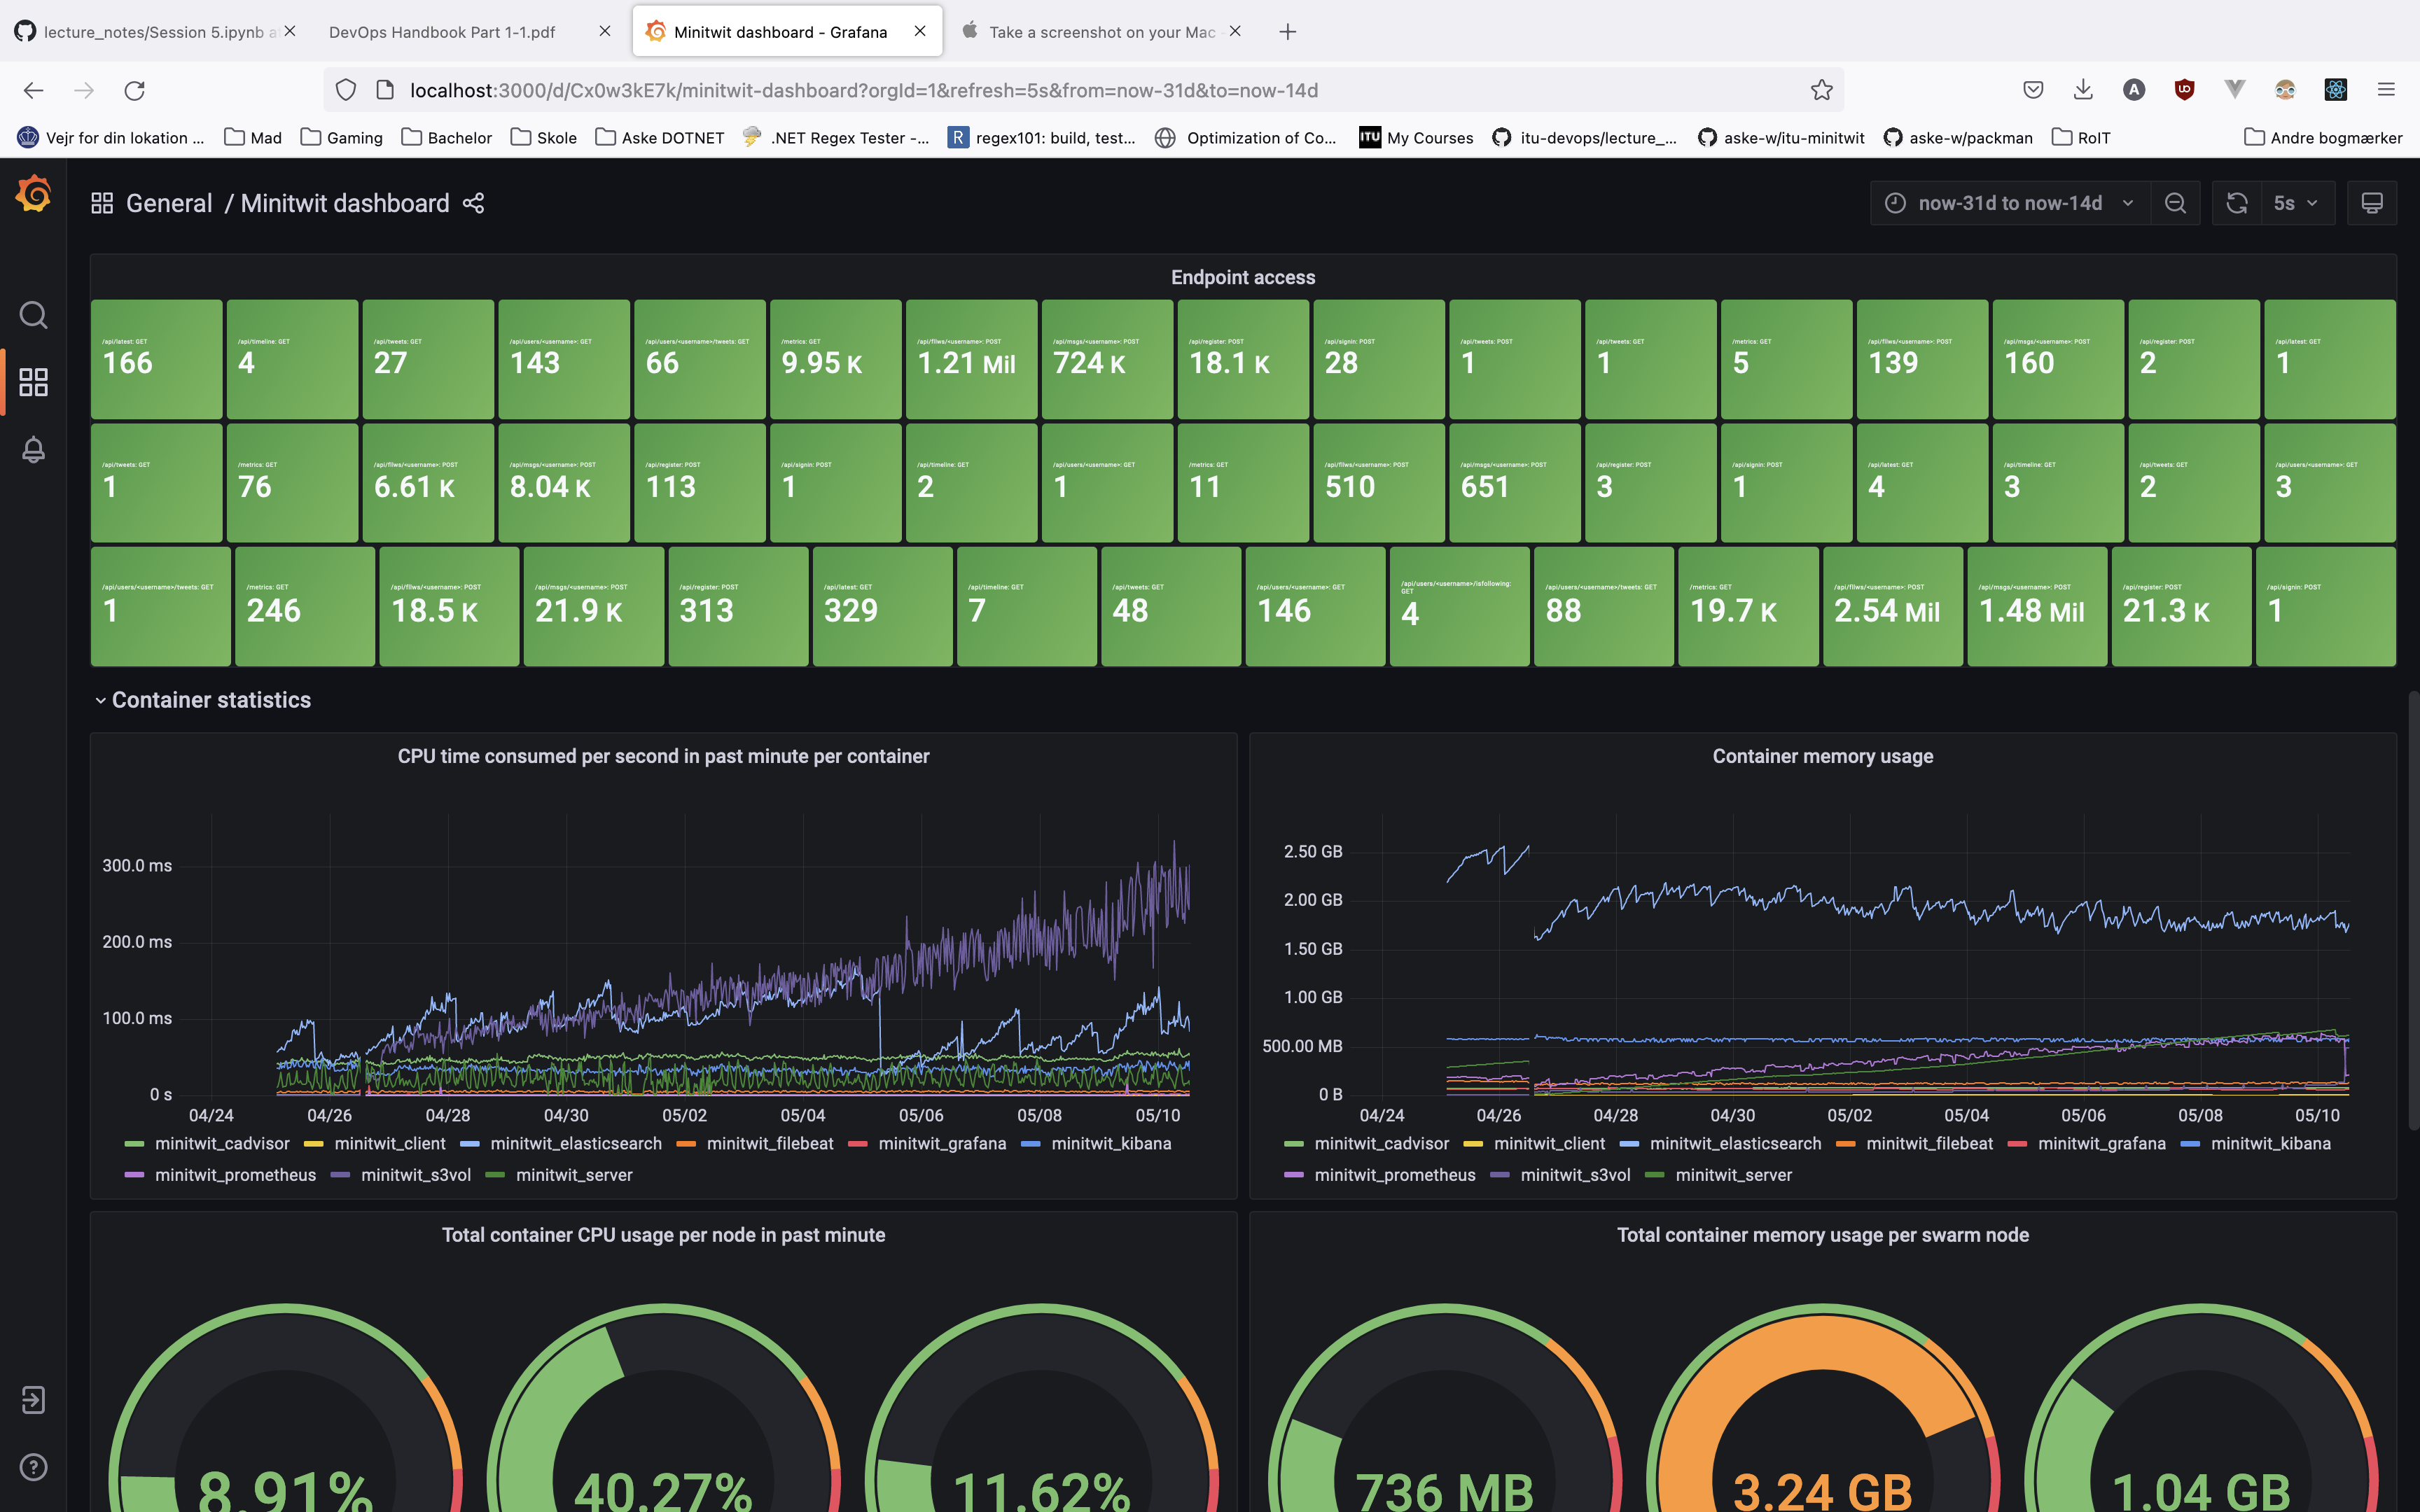
\includegraphics[height=0.6\textheight]{dashboard_2.png}
   }
   \caption{Screenshot of the Grafana dashboard showing the access count for each endpoint and CPU and memory statistics for containers}
   %\label{fig:gitguardian_email}
\end{figure}

\begin{figure}[H]
   \centering
   \rotatebox{90}{
        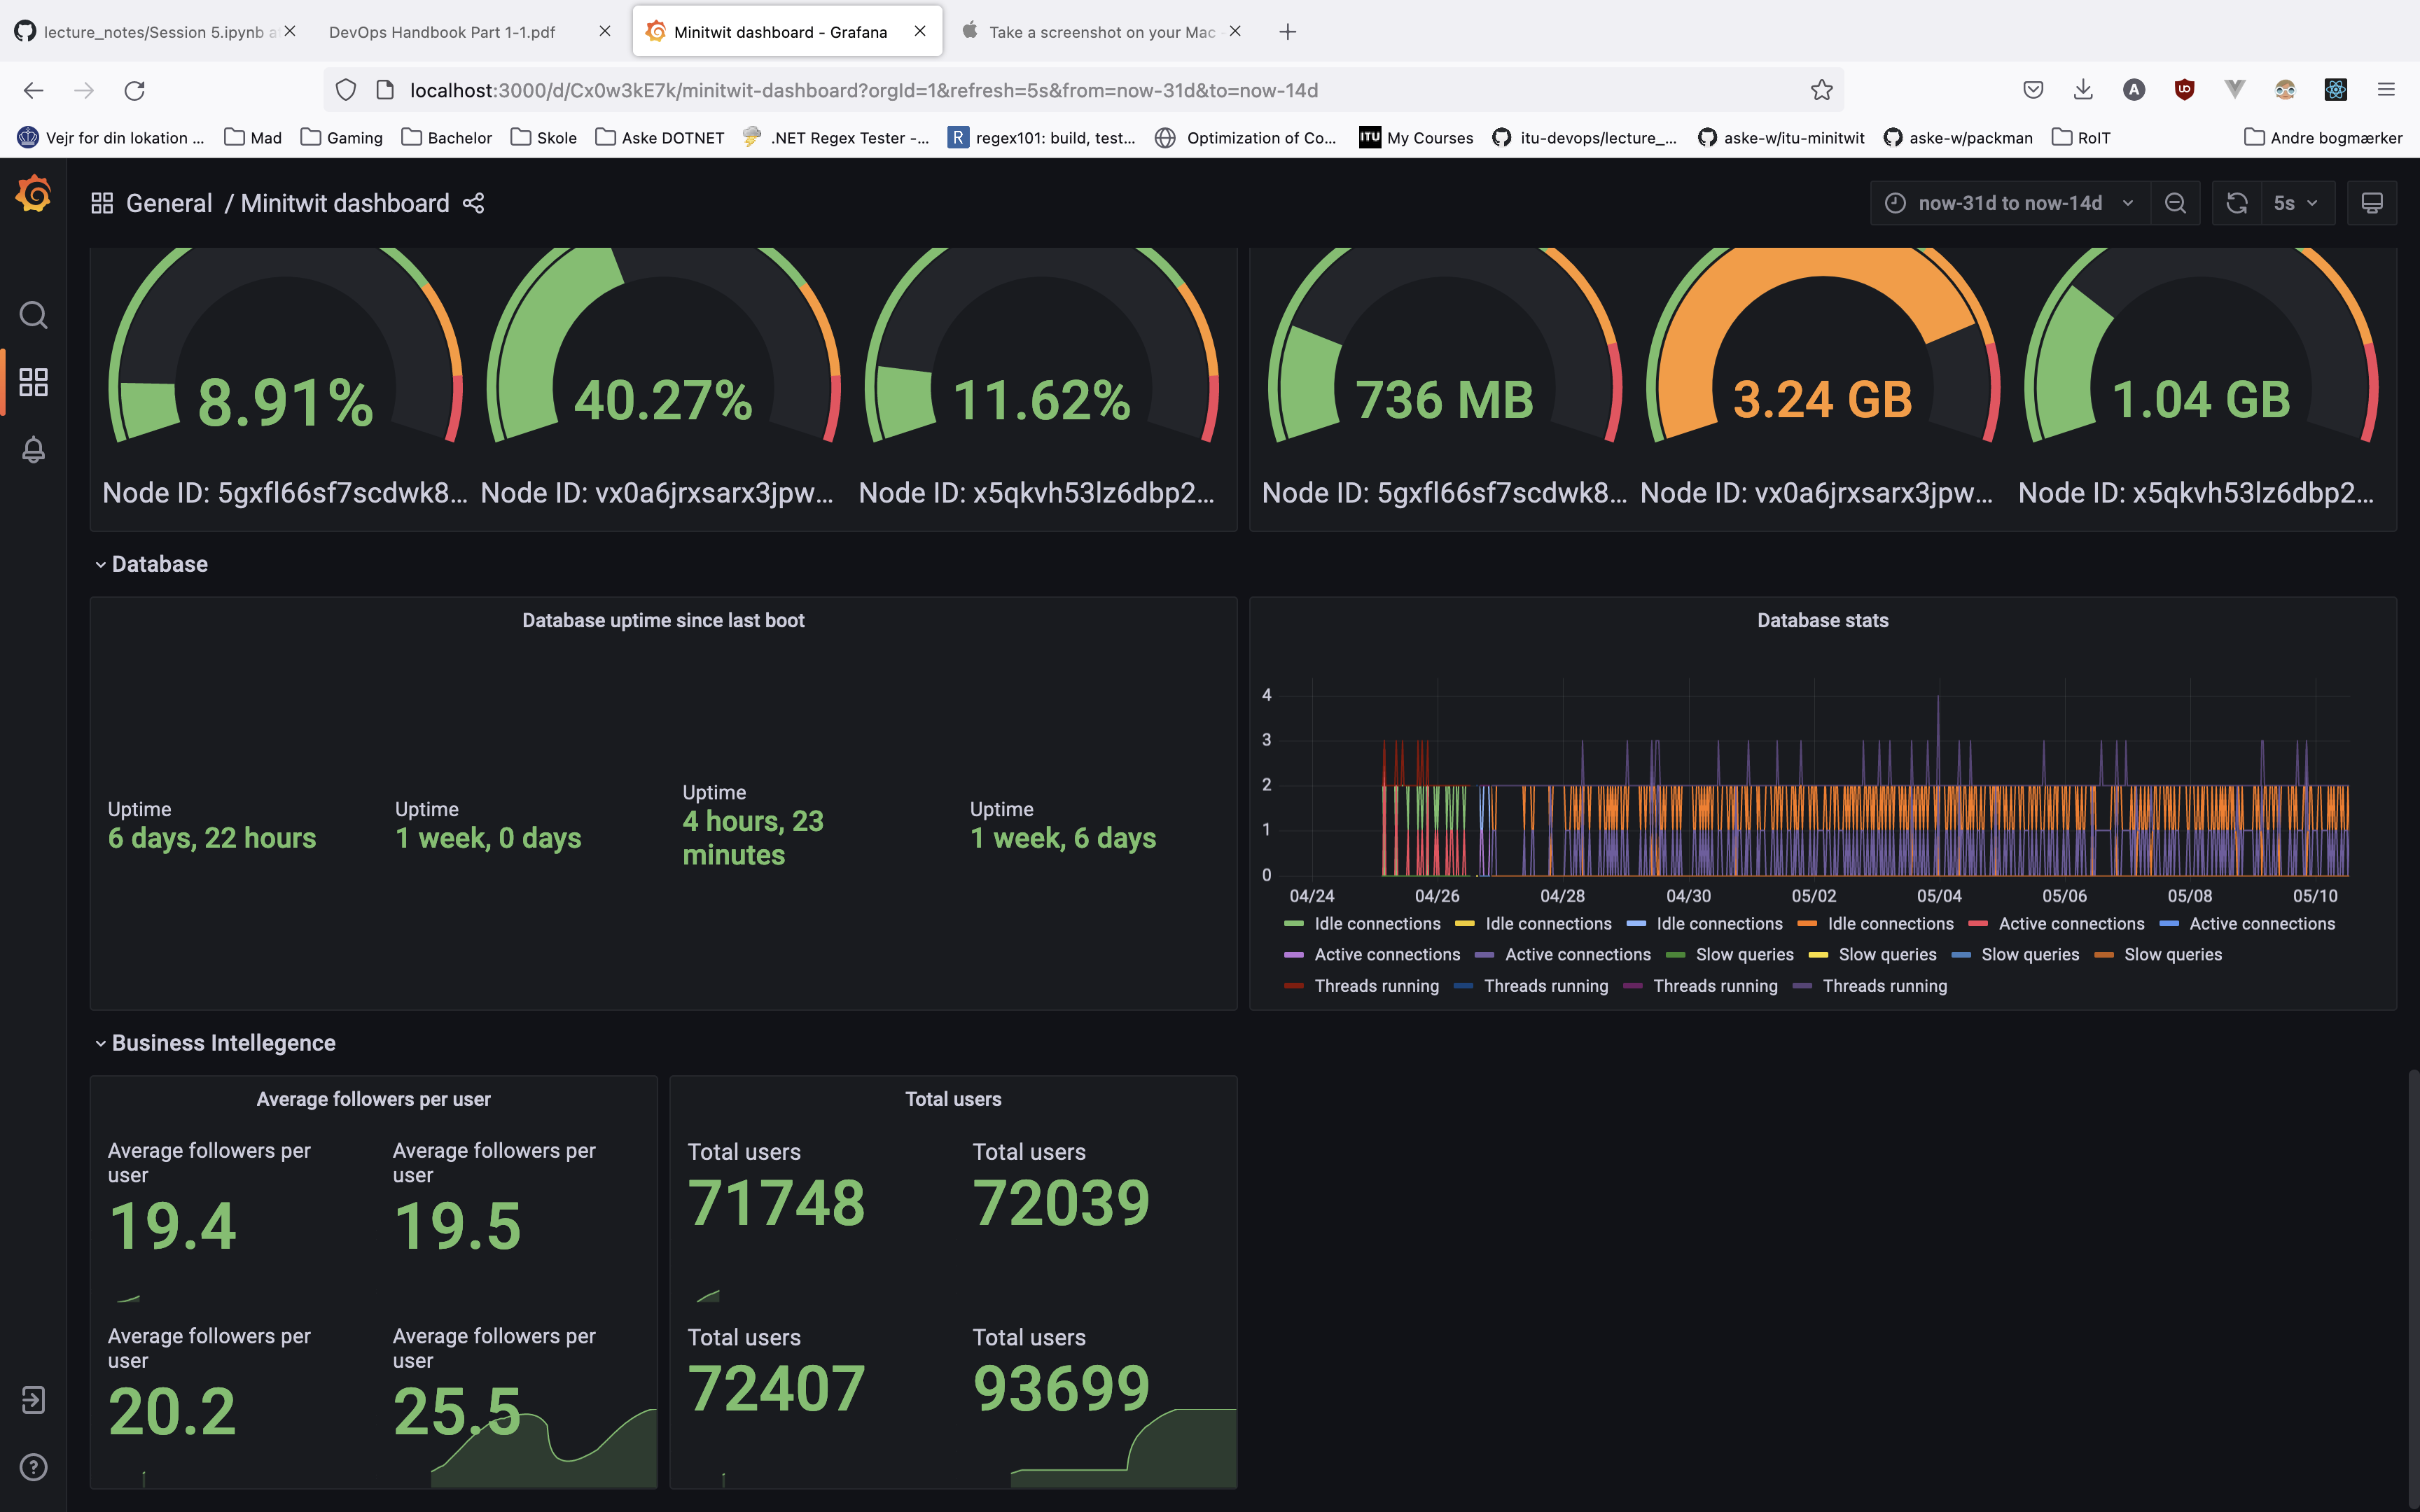
\includegraphics[height=0.6\textheight]{dashboard_3.png}
   }
   \caption{Screenshot of the Grafana dashboard showing the current memory and CPU usage for containers, database statistics and business intelligence}
   %\label{fig:gitguardian_email}
\end{figure}

\begin{figure}[H]
   \centering
    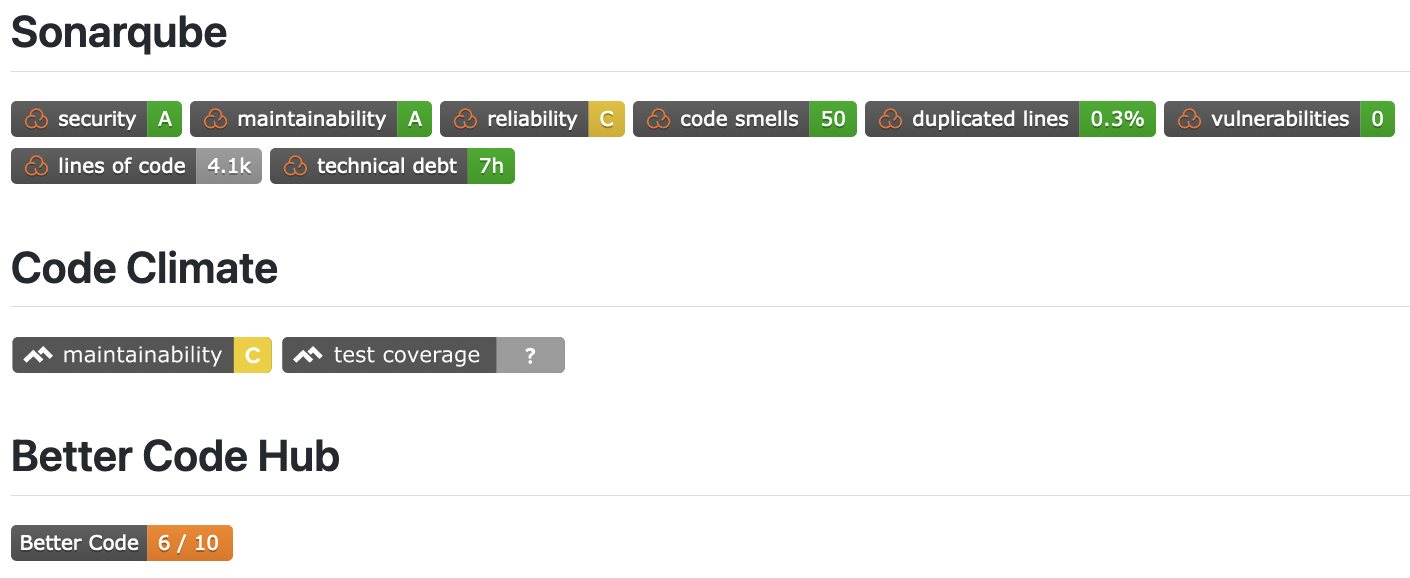
\includegraphics[width=\textwidth]{static analysis.png}
   \caption{Static analysis overview}
   \label{appendix:static_analysis}
\end{figure}
\newpage
\section{Lichen}
\label{appendix:lichen-output}
\begin{figure}[H]
   \centering
   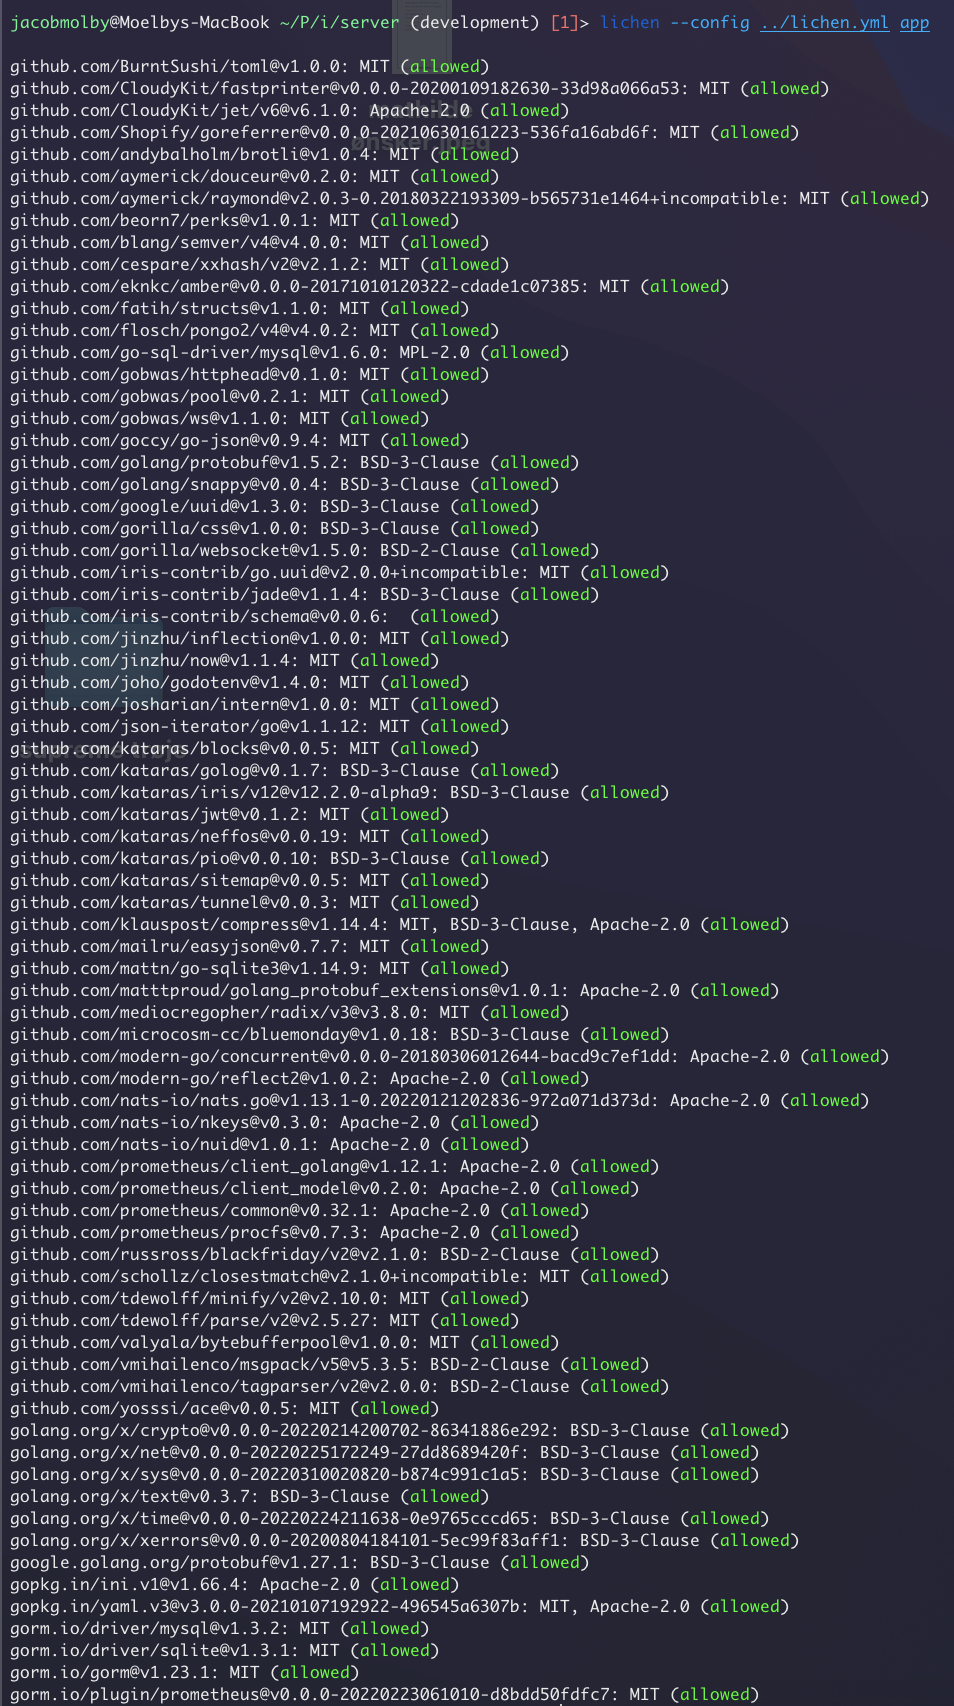
\includegraphics[height=0.85\textheight,keepaspectratio]{lichen.png}
   \caption{Output of Lichen}
   
\end{figure}



\end{document}
